\section{Pourquoi se conformer à un standard ? }
    \subsection{Un langage recommandé pour l’édition scientifique numérique}

Les corpus encodés en \TEI sont de plus en plus nombreux dans les projets de recherche en humanités numériques. La \TEI permet de préconiser des standards d'encodage au format \XML. Ces préconisations sont documentées dans les \textit{guidelines} disponibles en ligne et permettent d'assurer l'interopérabilité des données encodées en \XML pour l'édition scientifique numérique, en privilégiant un encodage sémantique afin de décrire les documents. Ce standard permet de s'adapter à un grand nombre de documents, nativement numériques ou transpositions de sources matérielles, et offre donc de nombreuses possibilités d'encodage et un niveau de personnalisation élevé, ce qui explique son utilisation de plus en plus majoritaire dans les projets d'édition scientifique numérique.

\begin{quote}
    La TEI met l’accent sur ce qui est partagé par tous les types de documents, qu’ils soient représentés physiquement sous une forme numérique sur un disque ou une carte mémoire, sous une forme imprimée comme un livre ou un journal, sous une forme écrite comme un manuscrit ou un codex, ou sous une forme inscrite dans la pierre ou sur une tablette de cire. Cette continuité facilite la migration du texte depuis des manifestations plus anciennes, comme l’imprimé ou le manuscrit, vers d’autres plus récentes comme le disque ou l’écran. \footnote{\cite{burnard_tei_2015}}
\end{quote}

En s'adaptant à tous types de documents, la \TEI représente un format de données idéal pour le projet \COREL : les textes de lois étant produits selon une architecture définie et régulière, ils se prêtent particulièrement bien à un encodage sémantique, qui permet de mettre en avant les éléments structurants des textes. De plus, la \TEI offre un vaste choix de balises, ce qui permet aux chercheurs du projets de pouvoir enrichir leurs sources, conformément aux objectifs du projet. Encoder les documents en \TEI garantit à la fois un encodage régulier et cohérent grâce à sa documentation, flexible et bien adapté aux sources grâce aux nombreuses possibilités d'encodage. Le passage à des documents encodés en \TEI, en plus de contribuer à l'interopérabilité des données de la recherche, assure aux chercheurs une indépendance dans les choix éditoriaux, contrairement au schéma figé du projet \LSC utilisé jusqu'à présent. Malgré la richesse de la \TEI, il est possible que l'utilisation de certains éléments ne correspondent pas entièrement aux spécificités d'un texte. Toutefois, ce cas de figure est également prévu par la \TEI. Il est en effet possible d'étendre le standard en modifiant le schéma d'encodage dans l'\ODD. Deux types de modifications de la \TEI sont alors possibles : des modifications dites \TEI \textit{conformant}, qui respectent les règles de la \TEI, ou bien des modifications qui outrepassent ces règles, bien que ces dernières ne soient pas conseillées. Que la \TEI soit étendue ou non, il est essentiel d'avoir un projet bien documenté, qui permette à d'autres utilisateurs de la \TEI de comprendre comment les données ont été structurées et quels choix d'encodage ont été faits. 

\subsection{Interopérabilité et documentation en ligne}

La \TEI a été créée en 1987 pour promouvoir un standard d'encodage des données en humanités numériques et ainsi permettre l'interopérabilité des ressources en ligne. En effet, le numérique apporte un foisonnement de données et de formats divers et souvent incompatibles entre eux, qui rendent l'échange des données difficile, voire impossible. Établir un standard de la diffusion des données en \textit{open access} afin de garantir leur accessibilité devient un enjeu majeur corrélé à l'apparition du web et à l'essor des formats propriétaires au profit des entreprises privées. Bien que les principes de science ouverte continuent de se développer aujourd'hui, il est primordial de maintenir la conformité à des standards afin de produire des données \fair et pérennes. 

L'encodage des données en \TEI permet ainsi de produire des données interopérables et réutilisables par la communauté de chercheurs en sciences humaines. C'est également un avantage pour l'équipe du projet, qui peut se référer aux \textit{guidelines} et accéder à une documentation claire et fournie, ce qui permet de faire des choix d'encodage adaptés et d'obtenir des documents \TEI valides. Cela permet aussi de se nourrir d'autres projets de recherche qui utilisent la \TEI et de pouvoir accéder à des outils de publication de données comme \tp. 
%parler un peu des exemples pris pour le projet ?

 \section{La transformation en XML-TEI}
    \subsection{Une transformation adaptée aux besoins du projet}
    
En plus de pouvoir s'appuyer sur des exemples de projets de recherche, encoder les documents du corpus en \TEI a permis d'établir un schéma d'encodage stable. En effet, les balises \TEI sont documentées dans les \textit{guidelines} et ont une utilisation prédéfinie, ce qui permet d'assurer la régularité de l'encodage au fur et à mesure du projet. Contrairement au schéma \LSC qui proposait une petite quantité de balises dont l'usage initial à été détourné au fil du temps, comme par exemple les balises \texttt{<content>}, un encodage en \TEI diminue le risque de mésusage des balises grâce à sa documentation. De plus, l'encodage du projet a pu s'écarter d'un schéma pensé pour l'affichage du texte afin d'adopter l'orientation sémantique de la \TEI. À court termes, cette pratique d'encodage offre une meilleure compréhension et structuration des documents, qui n'est plus liée à son affichage \HTML. À long termes, un encodage sémantique permet de produire un jeu de données qui pourra être réutilisé par les chercheurs, sans corrélation avec le projet \COREL. 

Il est pertinent de considérer les données comme un matériau à partir duquel le projet produit des livrables : si certains chercheurs en histoire du droit chinois consulteront le produit fini que sera le site web du projet, d'autres, initiés aux humanités numériques, pourront également consulter les données \TEI et les prendre comme support pour leurs propres recherches. Dissocier les données des livrables permet aussi d'enrichir les données de la recherche, puisque le projet \LSC notamment n'offre pas de données en libre-accès mais simplement les résultats produits à partir de ces données. Cette pratique d'un encodage sémantique, interopérable vient donc répondre à l'une des problématiques principales du projet au début du stage : la réutilisation de données produites pour un projet spécifique, qui ne respectent pas les principes \fair des données puisqu'elles ne sont pas disponibles en ligne librement (l'accès au site web \LSC est possible, mais les données ne sont pas mises à la disposition des chercheurs), non-interopérables car malgré le format d'encodage \XML, le schéma est entièrement personnalisé et non-documenté, ce qui aboutit enfin à des données qui peuvent difficilement être réutilisées. 
%peut-être conclure un peu mieux

\subsection{La transformation XSLT}

Le projet \cordel est l'un des exemples sur lequel le projet \COREL prend appui. Les données des deux projets présentent en effet des similarités. Issues de l'OCR, les données ont d'abord été encodées en \XML. Pour le projet \COREL, cet encodage provient d'un projet antérieur, tandis que pour le projet \cordel, les données de l'OCR ont été encodées automatiquement par \textit{Transkribus}. À l'instar de l'Université de Genève, les données des codes légaux chinois ont ensuite été transformée via le langage \XSLT en documents \TEI valides. 

Le langage \XSLT est un langage \XML conçu pour transformer des documents \XML en documents \XML, \HTML ou \LaTeX. Un document \XML en entrée passe par un processeur \XSLT avec des instructions \XSL rédigées dans une feuille de style.

\begin{figure}
    \centering
    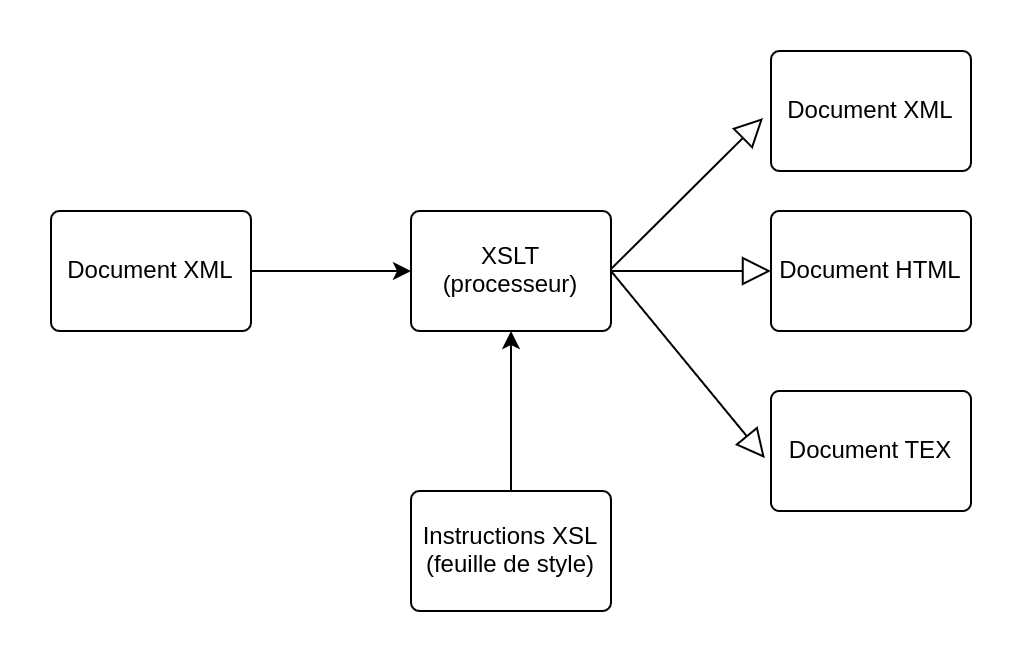
\includegraphics[width=\textwidth]{images/xslt.png}
    \caption{Modélisation de la transformation \XSLT}
\end{figure}
\newpage
Les données du projet \LSC conservent la structure générale des codes légaux chinois. Cela facilite la transformation \XSLT qui maintient cette structure en chapitres, sections et lois en sélectionnant uniquement les éléments structurants. Toutefois, l'une des difficultés de cette transformation, malgré la structure rigoureuse des textes chinois, découle de la modification des pratiques d'encodage dans le temps. En effet, puisque certaines balises sont utilisées selon des usages différents d'un document à l'autre, il est nécessaire de penser les règles de transformation avec de nombreuses exceptions. Ces contraintes ont donné lieu, dans un premier temps, à un code verbeux à l'intérieur duquel de nombreuses conditions \texttt{<xsl:if>} et \texttt{<xsl:when>} étaient imbriquées. Le code, en plus d'être difficile à lire, risquait de plus d'aboutir à des erreurs sur certaines de ces exceptions, erreurs difficilement repérables puisque je ne suis pas en mesure de lire les documents chinois. Dans ces circonstances, il est essentiel d'écrire un code qui soit le plus clair et simple possible, pour aboutir à un risque d'erreur faible. Le corpus étant composé d'un petit nombre de documents, une granularité fine de la feuille de style est envisageable, c'est pourquoi les règles de transformations ont été divisées en plusieurs éléments \texttt{<xsl:template>} : un template pour rédiger le \texttt{<teiHeader>} commun à tout le corpus puis un template pour chaque document du corpus. 

\begin{minted}{xslt}
    <!-- Nouveau template pour le code de 1740 -->
    <xsl:template match="/code[@id='DQLL1740']/document">
    ...
    </xsl:template>

    <!-- Nouveau template pour le code de 1646 -->
    <xsl:template match="/code[@id='code1646']/document">
    ...
    </xsl:template>
\end{minted}

%détailler le plus possible le processus de transformation, ce qui reste pareil ou non  (parler des div et des types, des identifiants qui ont été transformés en numérotation pour laisser la place à des identifiants uniques) expliquer que la séparation de chaque document, même si parfois un peu redondante, permet de faire des petits templates clairs et simples et d'éviter la multiplication des conditions (ici seulement 4 boucles pour chapitres/sections/lu/li).
